\section{Discete representation of continuos-Time signals}
\textbf{Fourier analysis} in general we can represent signals, continuos in the time domain, using a discrete representation in the frequency domain.
\[s(t) \overset{FS}{\Longleftrightarrow} S_k, \hspace{2em} k\in \mathbb{Z} \]
If the signal is periodic(\(T_0\)) and it has finite power \(P_s\):
\[s(t)=s(t-T_0)\hspace{1em}\forall t, \hspace{1em}P_s =\frac{1}{T_0}\int_{-T_0/2}^{T_0/2}|s(t)|^2 dt <+\infty\]
We can say:
\[s(t)=\sum_{k=-\infty}^{+\infty} S_k\cdot e^{j2\pi\frac{k}{T_0}t}\overset{FS}{\Longleftrightarrow}S_k=\frac{1}{T_0}\int_{-T_0/2}^{T_0/2}s(t)\cdot e^{-j2\pi\frac{k}{T_0}t}dt\]
\textbf{Bessel-Parseval formula}:
\begin{itemize}
    \item Power of \(s(t)\):\[P_s=\sum_{k=-\infty}^{+\infty}|S_k|^2\]
    \item Cross-power between \(s(t)\) and \(x(t)\): \[P_{sx}=\frac{1}{T_0}\int_{-T_0/2}^{T_0/2}s(t)x^*(t)dt=\sum_{k=-\infty}^{+\infty}S_kX_k^*\]
    \item Angle between \(s(t)\) and \(x(t)\):
    \[\theta= Angle(s(t),x(t))\rightarrow\cos\theta=\frac{Re\{P_{sx}\}}{\sqrt{P_sP_x}}\]
    \begin{itemize}
        \item If \(P_{sx}=0\rightarrow\cos\theta=0\rightarrow\) \(s(t)\) and \(x(t)\) are orthogonal
        \item \(\cos\theta =\pm 1\rightarrow\) \(s(t)\) and \(x(t)\) are collinear.
    \end{itemize}
\end{itemize}
\textbf{Discalimer}:
\begin{itemize}
    \item \texttt{Orthogonal}: dot product = 0
    \item \texttt{Collinear} : cross product = 0
\end{itemize}

If the signal in \textit{bandlimited}, the numbero of non-zero coefficients is finite.
EX:
\[
s(t)=A\cos(2\pi f_0t+\theta)\overset{FS}{\Longleftrightarrow}S_k=\begin{cases}
    \frac{A}{2}e^{j\theta}, \hspace{0.5em}k=1\\
    \ \frac{A}{2} e^{-j\theta}, \hspace{0.5em}k=-1\\
    0, \hspace{0.5em}{otherwise}
\end{cases}
\]
Also the power for the Bessel-Parseval equality:
\[
P_s=\sum_{k=-\infty}^{+\infty}|S_k|^2=\frac{A^2}{2}
\]
One of the fundamental properties in the frequency domain is that the convolution become a simple product(non ho voglia di riportare le formula)
(Questo per quanto visto mille volte rimane troppo importante)
\subsection{Sampling theorem}
First of all we need a: bandlimited finite-energy aperiodic signal.\\
\textbf{Whittaker-Shannon interpolation formula:}
\[s(t)=2B T_c\sum_{k=-\infty}^{+\infty}s(kT_c)\cdot \text{sinc}(2B(t-kT_c)), \text{where} \hspace{0.5 em}\text{sinc}(x)=\frac{\sin(\pi x)}{\pi x}\]
The perfect reconstruction of the signal \(s(t)\) from the samples can occur only if the Nysquist condition is satisfied(otherwise \textbf{Aliasing}):
\[
T_c\leq\frac{1}{2B}
\]
\subsection{Generalization}
In general the signal is defined as \underline{linear combination} of some predefined continuos-time functions(\textbf{signal expansion}:
\[
s(t)=\sum_{k=-\infty}^{+\infty} s_k\cdot\varphi_k(t)
\]
\begin{itemize}
    \item For finite-power periodic signals: Fourier
    \item For bandlimited finite-energy aperiodi signals: Whittaker
\end{itemize}
\subsection{Generalized fourier analysis or KLT}
\[
s(t)=\sum_{k=-\infty}^{+\infty}s_k\cdot\varphi_k(t)\overset{Basis}{\Longleftrightarrow}s_k
\]
L'insieme delle \(\varphi_k(t)\) are a set of predefined deterministic continuos-time signals called "basis", usually are orthornal.\\
The series of oefficients \(s_k\) represent the \textbf{image}.\\
If the basis are orthonormal:
\[
||\varphi_k(t)||_2=\sqrt{(\varphi_k(t),\varphi_k(t))^2}, \hspace{1em}(\varphi_k(t),\varphi_i(t))=\delta_{k,i}
\]
For this properties:
\[
s_k=(s(t),\varphi_k(t)), \forall k
\]
For example, for finite energy signals, the scalar product can be defined as the cross-energy between the two signals and the euclidean norm induced by the scalar product is the square root of the energy:
\[
(s(t),x(t))=\int_{-\infty}^{+\infty}s(t)x^*(t)dt=E_{sx}, \hspace{1em} ||s(t)||_2=\sqrt{(s(t),s(t))}=\sqrt{E_s}
\]
We can also define the distance between two signals:
\[
d(s(t),x(t))=||s(t)-x(t)||_2=\sqrt{(s(t)-x(t),s(t)-x(t))}
\]

For \textit{finite power periodic} signals:
\[
(s(t),x(t)) = \frac{1}{T_0}\int_{-T_0/2}^{T_0/2}s(t)x^*(t)dt = P_{sx}
\]
\textbf{Proof}
\begin{figure}[H]
    \centering
    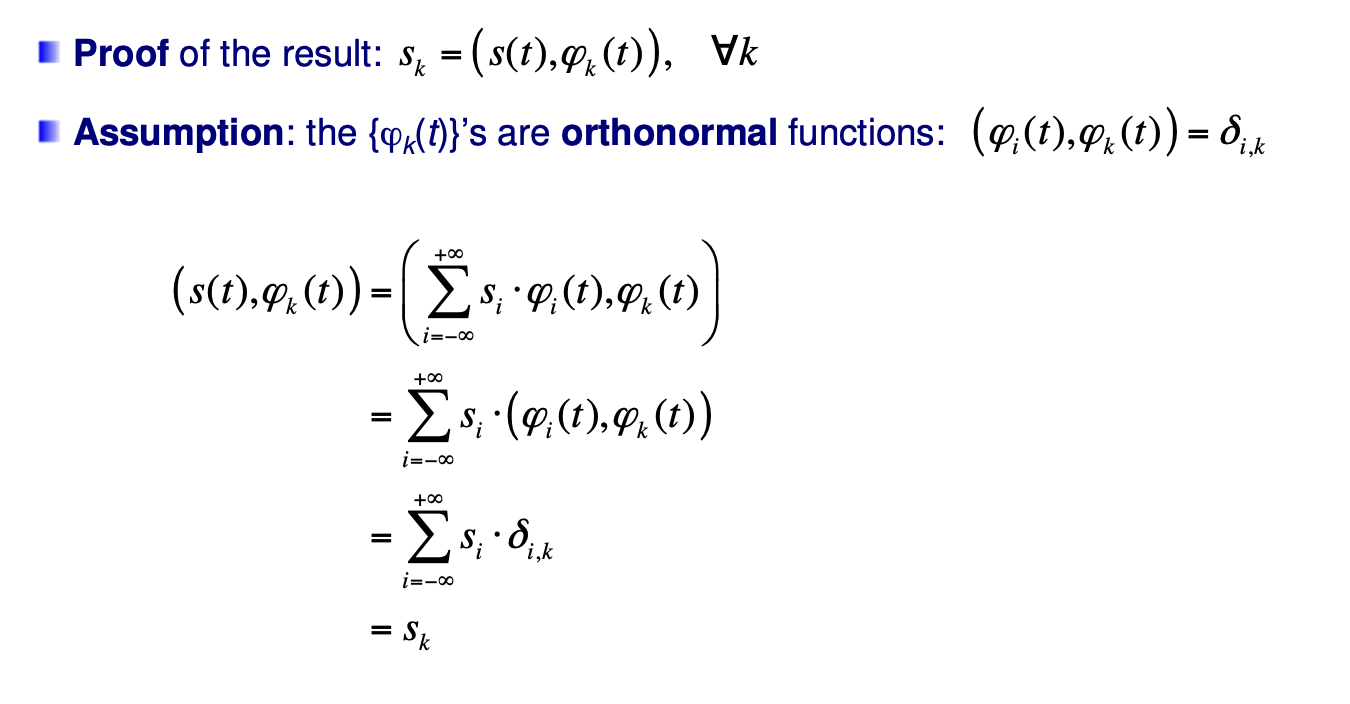
\includegraphics[width=1\linewidth]{Image/chap 1/1st_proof.png}
\end{figure}
This proof a property of the scalar product:
\[
(a\cdot s(t)+b\cdot q(t),\varphi (t))=a\cdot (s(t),\varphi_k(t)+b\cdot (q(t),\varphi (t))
\]
\texttt{Important}: if the signals are expanded on an orthonormal basis, the scalar product between two signals and their norms can be obtained by processing the image vector as well:
\begin{figure}[H]
    \centering
    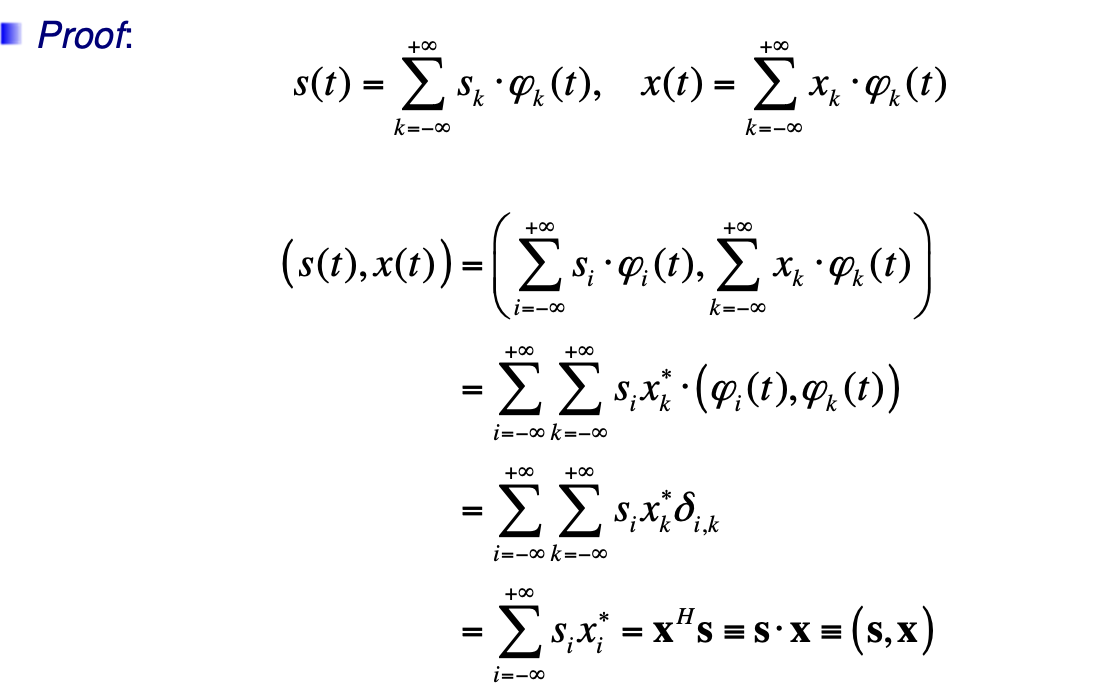
\includegraphics[width=1\linewidth]{Image/chap 1/2nd_proof.png}
\end{figure}
From this point on, if we we have the scalar product we adopt:
\[
(s(t),x(t))=(\mathbf{s},\mathbf{x})
\]
If we assume \(x(t)=s(t)\), we also get:
\[
||s(t)||_2^2=||s||_2^2
\]
\textbf{In summary}: if the signals are expanded on an orthonormal basis, the scalar product between two signals and their norm can be obtained by processing the image vectors instead of processing the continuos-time signal, the Bessel-Parseval equality for Fourier series is a particular case:
\[
||s(t)||_2^2=\frac{1}{T_0}\int_{-T_0/2}^{T_0/2}|s(t)|^2dt=\sum_{k=-\infty}^{+\infty}|S_k|^2=||s||_2^2
\]
When observe a signal we are considering just a part of the signal, if we suppose it continuos. So is like observing a signal \(s(t)\) for \(t\in [0,T]\), so is like multiplying for a rect function:
\[
s(t)=A\cdot \text{rect}\left(\frac{t-T/2}{T}\right)\Longleftrightarrow S(f)=AT\cdot \text{sinc}(fT)e^{-j\pi fT}
\]
Remember that \(s(t)\) is supposed with an infinite band-width.\\
The Energy spectral density is:
\[
ESD(f)=|S(f)|^2
\]
The energy of the signal:
\[
E_s=\int_{-\infty}^{+\infty} |S(f)|^2 df
\]
Even if the signal is infinite-bandwidth, most of the energy is in a defined bandwidth \(B\):
\[
E_b=\int_{-B}^{B} |S(f)|^2df
\]
If \(B\) is large enough: \[
E_b\approx E_x
\]
Right now is trying to represent a the below signal in a discrete way using the Whitaker-interpolation formula:
\begin{figure}[H]
    \centering
    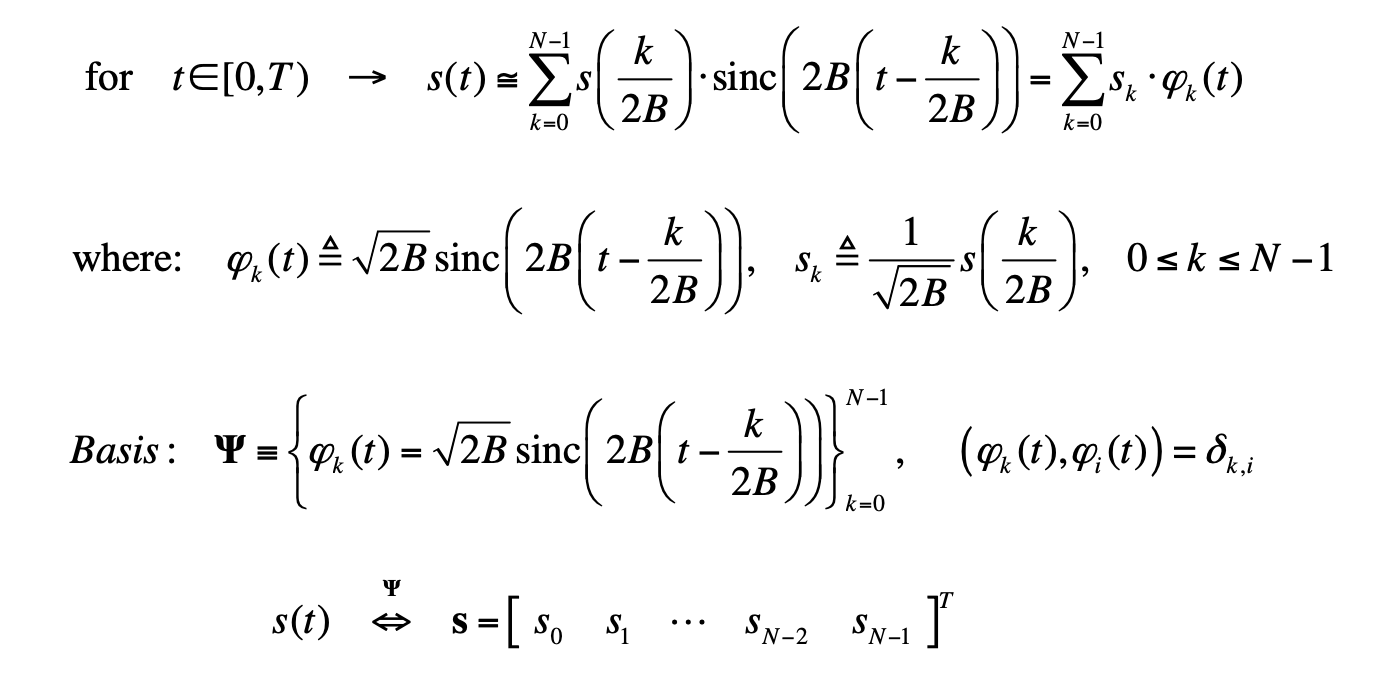
\includegraphics[width=1\linewidth]{Image/chap 1/3rd_scheme.png}
\end{figure}
To see if the approximation used is good we need to study the error:
\[
s_{\Delta}(t) = s(t)-\hat{s}(t)
\]
If B is large enough, such that:
\[
N=\frac{T}{T_c}=2BT\gg 1
\]
\[
\text{then } E_{\Delta}\leq \alpha E_s\text{ with }\alpha\ll 1
\]
In this case, we say that \(X(t)\) has essential bandwidth \(B\) at level \(\alpha \) and \(B\) is the essential bandwidth at level \(\alpha\) of the signal \(X(t)\), so essentially the most of energy is stored in this bandwidth.
\subsection{The discrete Karhunen-Loeve Transform(DKLT)}
\subsubsection{Basis expansion of discrete-time signals}
Nowadays the tendency is to sample the signal as soon as possible in the processing chain.\\
If \(T\) is the observation interval and B the bandwidth of the signal(after an anti-aliasing filter), we have seen that if \(T_c\leq1/(2B)\) and \(N=T/T_c\gg1\), we have :
\[
    X(t) \cong 2BT_{c} \sum_{k=0}^{N-1} X(kT_{c}) \cdot \operatorname{sinc}(2B(t-kT_{c})), \quad t \in [0, T]
\]

\[
    \Psi \equiv \left\{ \varphi_{k}(t) = \sqrt{2B} \ \operatorname{sinc} \left(2B(t-kT_{c})\right) \right\}_{k=0}^{N-1}, \qquad N = \frac{T}{T_{c}}
\]

\[
    X(t) {\xLeftrightarrow{\Psi}} \mathbf{X} = \frac{2BT_c}{\sqrt{2B}}
    \begin{bmatrix}
        X(0) & X(T_c) & \cdots & X((N-1)T_c)
    \end{bmatrix}^{T}
\]

\noindent If we choose the \textit{Nyquist sampling interval} \(T_c=1/2B\) we have:

\[
\Psi \equiv \left\{
    \varphi_k(t) = \sqrt{2B} \; \mathrm{sinc}\left(2B\left(t - \frac{k}{2B}\right)\right)
\right\}_{k=0}^{N-1}, \qquad
N = \frac{T}{T_c} = 2BT
\]
The finite-energy discrete-time signal we obtain by sampling is:
\[
\mathbf{X} = 
\begin{bmatrix}
    X[0] & X[1] & \cdots & X[N-1]
\end{bmatrix}^{T},
\quad \text{where} \quad 
X[n] \triangleq \frac{1}{\sqrt{2B}}\, X\left(\frac{n}{2B}\right)
\]

\noindent \(N=2BT\gg 1\) is the dimension of the image vector and we also say that \(N\) is the dimension of the continuos-time signal \(X(t)\).


\noindent In many cases, it can be useful to expand the discrete-time signal obtained by sampling into a set of deterministic \underline{discrete-time orthonormal basis} function as follows:
\[
X[n] = \sum_{i=0}^{K-1} \alpha_i \varphi_i[n], \quad n = 0, 1, \ldots, N-1; \quad K \leq N
\]

\noindent The basis is orthonormal if:\\
\[
\left( \varphi_i[n], \varphi_k[n] \right) = \delta_{i,k} = 
\begin{cases}
    1, & k = i \\
    0, & k \neq i
\end{cases}
\]
\noindent Note that if \(K<N\) the expansion represents a \textit{data compression}:
\[
\underset{N\times1}{\mathbf{X}} \xLeftrightarrow{\Psi} \underset{K\times1}{\boldsymbol{\alpha}}
\]
REMEMBER: the idea is to find \(K\ll N\).

In the case of finite duration \(N\), i.e finite-energy, discrete time signals, the \textbf{inner product} and the induced \textbf{Euclidean norm} can be defined as follows:
$$
\left( s[n], x[n] \right) \triangleq \sum_{n=0}^{N-1} s[n] x^{*}[n] = E_{sx}\qquad(\text{cross-energy})
$$

\[
    \|s[n]\|_{2} \triangleq \sqrt{(s[n], s[n])} = \sqrt{\sum_{n=0}^{N-1} |s[n]|^{2}} = \sqrt{E_{s}} \qquad \left(\sqrt{\text{energy}}\right)
\]

The coefficients in the expansion are derived as the inner product between \(X[n]\) and the basis functions :
$$
\alpha_i = (\mathbf{X}[n], \varphi_i[n]) = \sum_{n=0}^{N-1} X[n]\, \varphi_i^{*}[n] = \varphi_i^{H} \mathbf{X}, \quad i = 0, 1, \ldots, K-1
$$
\begin{figure}[H]
    \centering
    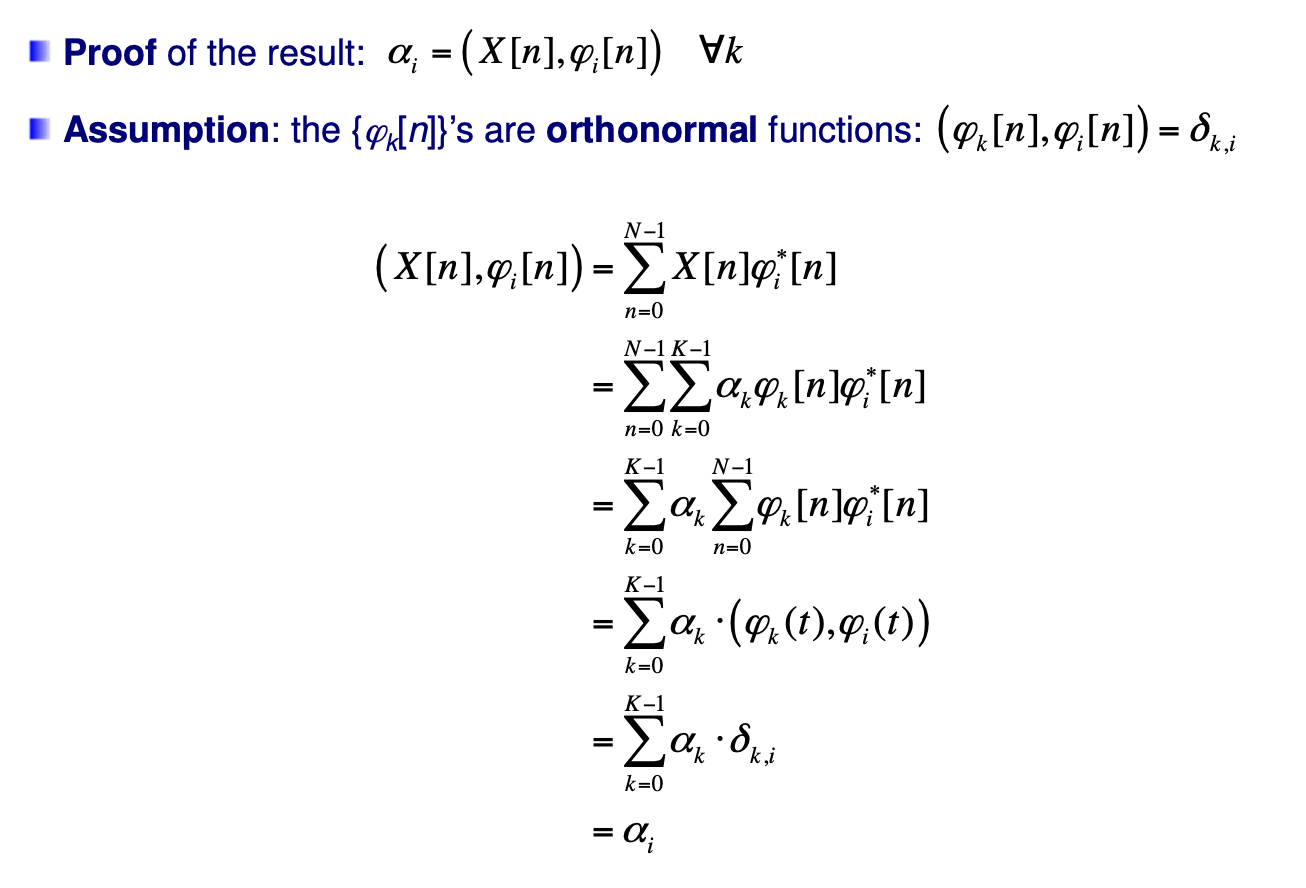
\includegraphics[width=0.5\linewidth]{Image/chap 1/5. 4th proof.png}
\end{figure}
\textbf{Problem}: which is the choice of the basis that makes the coefficients \(\alpha_i\) \underline{uncorrelated}? Remember that if \(X(t)\) is a random process the coefficients are r.v.'s
\[
\mathbf{X} = \begin{bmatrix} X[0] & X[1] & \cdots & X[N-1] \end{bmatrix}^{T}_{N \times 1}
\]

\[
\boldsymbol{\alpha} = \begin{bmatrix} \alpha_0 & \alpha_1 & \cdots & \alpha_{K-1} \end{bmatrix}^{T}_{K \times 1}
\]

\[
\boldsymbol{\varphi}_i = \begin{bmatrix} \varphi_i[0] & \varphi_i[1] & \cdots & \varphi_i[N-1] \end{bmatrix}^{T}_{N \times 1}
\]

\[
\left(\varphi_k[n],\, \varphi_i[n]\right) = (\varphi_k,\, \varphi_i) = \varphi_i^{H} \varphi_k = \delta_{i,k}
\]

\[
\mathbf{\Phi} = \begin{bmatrix} \varphi_0 & \varphi_1 & \cdots & \varphi_{K-1} \end{bmatrix}_{N \times K}, \qquad 
\text{if } K = N \Rightarrow \text{unitary matrix,} \quad \mathbf{\Phi}^{-1} = \mathbf{\Phi}^{H}
\]

\noindent Which is the choice of the basis that makes the coefficients \(\alpha_i\), uncorrelated?\\
\noindent Assume \(K=N\) and, without loss of generality, also that \(E\{X[n]\}=0\rightarrow E\{\alpha_i\}=0\).
\[
X[n] = \sum_{i=0}^{N-1} \alpha_i \varphi_i[n], \qquad n = 0, 1, \ldots, N-1
\]

\[
\mathbf{X} = \sum_{i=0}^{N-1} \alpha_i \boldsymbol{\varphi}_i = \mathbf{\Phi} \boldsymbol{\alpha}
\qquad \Rightarrow \qquad
\mathbf{\Phi}^H \mathbf{X} = \mathbf{\Phi}^H \mathbf{\Phi} \boldsymbol{\alpha} = \boldsymbol{\alpha}
\]

\[
\mathbf{\Phi} : \quad E\left\{ \boldsymbol{\alpha} \boldsymbol{\alpha}^H \right\} = 
\begin{bmatrix}
\sigma_0^2 & 0 & \cdots & 0 \\
0 & \sigma_1^2 & \cdots & 0 \\
\vdots & \vdots & \ddots & \vdots \\
0 & 0 & \cdots & \sigma_{N-1}^2
\end{bmatrix}
= \mathbf{\Lambda}, \qquad
\text{where} \quad \sigma_i^2 \triangleq E\left\{ |\alpha_i|^2 \right\}
\]

\[
\text{and} \qquad E\left\{ \alpha_i \alpha_k^* \right\} = 0 \qquad \text{if } i \ne k
\]
\newpage
\[
\mathbf{\Phi} : \quad E \left\{ \boldsymbol{\alpha} \boldsymbol{\alpha}^H \right\} 
= E \left\{ \mathbf{\Phi}^H \mathbf{X} \mathbf{X}^H \mathbf{\Phi} \right\}
= \mathbf{\Phi}^H E \left\{ \mathbf{X} \mathbf{X}^H \right\} \mathbf{\Phi}
= \mathbf{\Phi}^H \mathbf{R}_X \mathbf{\Phi}
= \mathbf{\Lambda}
\]
\[
\mathbf{\Lambda} = \mathbf{\Phi}^H \mathbf{R}_X \mathbf{\Phi}
\implies
\mathbf{\Phi} \mathbf{\Lambda} \mathbf{\Phi}^H = \mathbf{\Phi} \mathbf{\Phi}^H \mathbf{R}_X \mathbf{\Phi} \mathbf{\Phi}^H
\implies
\mathbf{R}_X = \mathbf{\Phi} \mathbf{\Lambda} \mathbf{\Phi}^H
\]
\begin{itemize}
    \item Matrix \(\mathbf{\Phi}\) diagonalizes the correlation matrix \(\mathbf{R}_X\rightarrow\) the basis that makes the coefficients uncorrelated is obtained from the \textbf{Eigenvector-Eigenvalue Decomposition(EVD)} of the correlation matrix \(\mathbf{R}_X\) of the random vector \(\mathbf{X}\rightarrow\Phi\) is formed by the eigenvectors of \(\mathbf{R}_X\).
    \item The expansion on this basis is called \textbf{Karhunen-Loève expansion} and the vector of coefficients \(\alpha\) is called \textbf{discrete Karhunen-Loève expansion} and the vector of coefficients \(\alpha\) is called \textbf{DKLT}.
    \item Definition of the correlation matrix \(\mathbf{R}_X\) of a random vector \(\mathbf{X}\):
\[
\mathbf{R}_X \triangleq E \left\{ \mathbf{X} \mathbf{X}^H \right\} 
= E \left\{
\begin{pmatrix}
X_1 \\
X_2 \\
\vdots \\
X_N
\end{pmatrix}
\begin{pmatrix}
X_1^{*} & X_2^{*} & \cdots & X_N^{*}
\end{pmatrix}
\right\}
= E \left\{
\begin{pmatrix}
|X_1|^2 & X_1 X_2^{*} & \cdots & X_1 X_N^{*} \\
X_2 X_1^{*} & |X_2|^2 & \cdots & X_2 X_N^{*} \\
\vdots & \vdots & \ddots & \vdots \\
X_N X_1^{*} & X_N X_2^{*} & \cdots & |X_N|^2
\end{pmatrix}
\right\}
\]
\[
\hspace{-4.25em}\mathbf{R}_X =
\begin{bmatrix}
    E \left\{ |X_1|^2 \right\} & E \left\{ X_1 X_2^* \right\} & \cdots & E \left\{ X_1 X_N^* \right\} \\
    E \left\{ X_2 X_1^* \right\} & E \left\{ |X_2|^2 \right\} & \cdots & E \left\{ X_2 X_N^* \right\} \\
    \vdots & \vdots & \ddots & \vdots \\
    E \left\{ X_N X_1^* \right\} & E \left\{ X_N X_2^* \right\} & \cdots & E \left\{ |X_N|^2 \right\}
\end{bmatrix}
=
\begin{bmatrix}
    E \left\{ |X_1|^2 \right\} & E \left\{ X_1 X_2^* \right\} & \cdots & E \left\{ X_1 X_N^* \right\} \\
    \left( E \left\{ X_1 X_2^* \right\} \right)^* & E \left\{ |X_2|^2 \right\} & \cdots & E \left\{ X_2 X_N^* \right\} \\
    \vdots & \vdots & \ddots & \vdots \\
    \left( E \left\{ X_1 X_N^* \right\} \right)^* & \left( E \left\{ X_2 X_N^* \right\} \right)^* & \cdots & E \left\{ |X_N|^2 \right\}
\end{bmatrix}
= 
\mathbf{R}_X^H
\]
\end{itemize}
If the data vector \(\mathbf{X}\) is obtained by sampling a continuos-time wide-sense stationary (w.s.s) process \(X(t)\):
\[
X_{i+1} \triangleq [\mathbf{X}]_{i+1} = X[i] = \frac{1}{\sqrt{2B}} X\left( \frac{i}{2B} \right), \quad i = 0, 1, 2, \ldots, N-1
\]

\[
[\mathbf{R}_X]_{i+1,j+1} = E\left\{ X_{i+1} X_{j+1}^* \right\} = E\left\{ X[i] X^*[j] \right\} = R_X[j-i]
\]

\[
= \frac{1}{2B} E\left\{ X\left( \frac{i}{2B} \right) X^*\left( \frac{j}{2B} \right) \right\}
= \frac{1}{2B} R_X\left( \frac{j-i}{2B} \right)
\]

\[
i, j = 0, 1, 2, \ldots, N-1
\]
Hence, if the data vector \(\mathbf{X}\) is obtained by sampling a continuous-tim w.s.s process \(X(t)\) with autocorrelation function (ACF):
\(
R_X(\tau)=E\{X(t)X^*(t+\tau)\}
\),
in addition to be hermitian, the correlation of \(\mathbf{X}\) has a \underline{Toeplitz} structure:
\[
\mathbf{R}_X = \frac{1}{2B}
\begin{bmatrix}
    R_X(0) & R_X\left(\frac{1}{2B}\right) & R_X\left(\frac{2}{2B}\right) & \cdots & R_X\left(\frac{N-2}{2B}\right) & R_X\left(\frac{N-1}{2B}\right) \\
    R_X^*\left(\frac{1}{2B}\right) & R_X(0) & R_X\left(\frac{1}{2B}\right) & \cdots & R_X\left(\frac{N-3}{2B}\right) & R_X\left(\frac{N-2}{2B}\right) \\
    R_X^*\left(\frac{2}{2B}\right) & R_X^*\left(\frac{1}{2B}\right) & R_X(0) & \cdots & R_X\left(\frac{N-4}{2B}\right) & R_X\left(\frac{N-3}{2B}\right) \\
    \vdots & \vdots & \vdots & \ddots & \vdots & \vdots \\
    R_X^*\left(\frac{N-2}{2B}\right) & R_X^*\left(\frac{N-3}{2B}\right) & R_X^*\left(\frac{N-4}{2B}\right) & \cdots & R_X(0) & R_X\left(\frac{1}{2B}\right) \\
    R_X^*\left(\frac{N-1}{2B}\right) & R_X^*\left(\frac{N-2}{2B}\right) & R_X^*\left(\frac{N-3}{2B}\right) & \cdots & R_X^*\left(\frac{1}{2B}\right) & R_X(0)
\end{bmatrix}
\]
The \textbf{DKLT} is a \textbf{linear whitening(decorrelating) transformation} of the original data vector \(\mathbf{X}\):
\[
\underset{N\times1}{\mathbf{X}}\xLeftrightarrow{DKLT}\underset{N\times1}{\boldsymbol{\alpha}}
\]
\[
\boldsymbol{\alpha}=\boldsymbol{\Phi}^H\mathbf{X}
\]


\[
\mathbf{\Phi}:\quad E\left\{ \boldsymbol{\alpha}\boldsymbol{\alpha}^H \right\} =
\begin{bmatrix}
\sigma_0^2 & 0 & \cdots & 0 \\
0 & \sigma_1^2 & \cdots & 0 \\
\vdots & \vdots & \ddots & \vdots \\
0 & 0 & \cdots & \sigma_{N-1}^2
\end{bmatrix},
\quad \text{where} \quad
\sigma_i^2 \triangleq E\left\{|\alpha_i|^2\right\}
\]

\noindent In many receivers, the first operation that is perfomed is a linear whitening transformation of the data vector \textbf{X}.
\begin{itemize}
    \item The \textbf{DKLT} of the original data vector \textbf{X} requires knowledge of the correlation matrix \(\textbf{R}_X\) of a random vector \textbf{X}, i.e pf the ACF of the w.s.s process \(X(t)\).
    \item \(\Phi\) is obtained from the \textbf{Eigenvector-Eigenvalue Decomposiition(EVD)} of the correlation matrix \(\textbf{R}_X\rightarrow\Phi\) is formed by the eigenvectors of \(\textbf{R}_X\):
    \[
    \mathbf{R}_X=\mathbf{\Phi\Lambda\Phi}^H
    \]
    \item In many applications, we do not know a priori the correlation matrix \(\mathbf{R}_X\), so we have to estimate it from the data:
    \[
    \mathbf{\hat{R}}\Rightarrow(\mathbf{\hat{\Phi}},\mathbf{\hat{\Lambda}})\hspace{0.5em}\text{from the EVD of }\mathbf{\hat{R}}_X:\hspace{0.5em}\mathbf{\hat{R}}=\mathbf{\Phi\Lambda\Phi}^H    \]
    \item  We will see later on how to \underline{estimate the correlation matrix} of a \(N-\)dimensional random vector \textbf{X} given a number \(M>N\) of independent realizations of \textbf{X}.
\end{itemize}
Changing of the base:
\begin{itemize}
    \item \(\Phi\) is a unitary matrix and \(\alpha=\Phi^H\mathbf{X}\) is a linear transformation of the data.
    \item It is basically a rotation of the reference system in such a way that the components in the new reference system are uncorrelated:
    \begin{figure}[H]
        \centering
        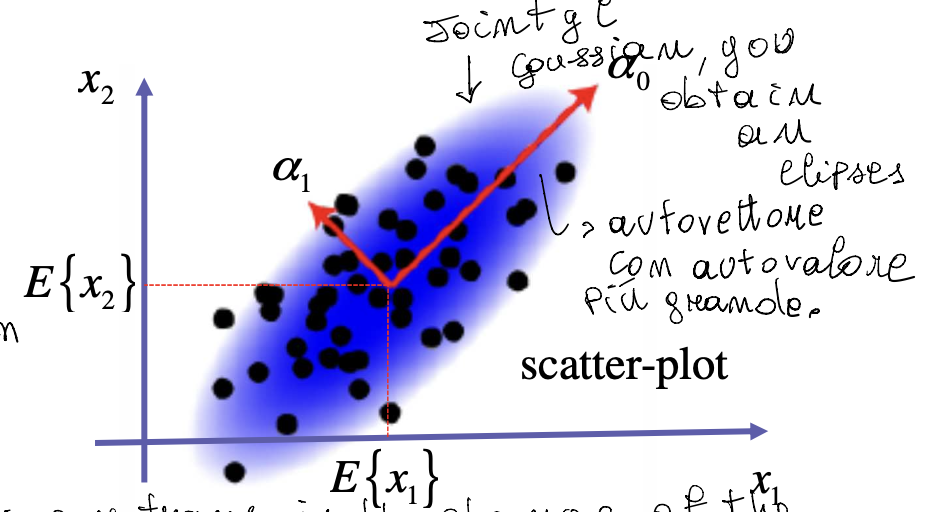
\includegraphics[width=0.5\linewidth]{Image/chap 1/6. Scatter_plot.png}
        \label{fig:placeholder}
    \end{figure}
    \item if \textbf{X} is non-zero mean, we can remove the mean, and \(\Phi\) is obtained by the EVD of the \underline{covariance matrix} of vector \textbf{X}.
    \[\boldsymbol{\alpha}=\boldsymbol{\Phi}^H(\mathbf{X}-\mathbf{m}_X)\]
    \[
    \text{where}\hspace{0.35em}\textbf{m}_X\triangleq E\{\mathbf{X}\}\]
    \[
\mathbf{\Phi} : \quad
\mathbf{C}_X \triangleq E \left\{ (\mathbf{X} - \mathbf{m}_X)(\mathbf{X} - \mathbf{m}_X)^H \right\} = \mathbf{\Phi} \mathbf{\Lambda} \mathbf{\Phi}^H
\]

    \item \textbf{IMPORTANT}: it is well-known that if the correlation time \(L\) of the discrete-time sequence \(X[n]\) is much lower than the vector size \(N\), then the matrix \(\Phi\) that diagonalizes the correlation matrix \(\textbf{R}_X\) is (approximately) the DFT matrix and the DKLT coincides with the (unitary) DFT:
    \[
L \ll N \qquad \Rightarrow \qquad
\varphi_i[n] \cong \frac{1}{\sqrt{N}} e^{j 2 \pi \frac{i}{N} n} 
\qquad ; \quad i, n = 0, 1, \ldots, N-1
\]
\[
\mathbf{X} = \mathbf{\Phi} \boldsymbol{\alpha} \cong \text{IDFT}\{\boldsymbol{\alpha}\}
\iff
\boldsymbol{\alpha} = \mathbf{\Phi}^H \mathbf{X} \cong \text{DFT}\{ \mathbf{X} \}
\]
\[
X[n] \cong \frac{1}{\sqrt{N}} \sum_{i=0}^{N-1} \alpha_i e^{j 2 \pi \frac{i}{N} n}
\]
\[
\alpha_i = (X[n], \varphi_i[n]) \cong \frac{1}{\sqrt{N}} \sum_{n=0}^{N-1} X[n] e^{-j 2 \pi \frac{i}{N} n}
\]
\[
\mathbf{\Phi} = \frac{1}{\sqrt{N}}
\begin{bmatrix}
1 & 1 & \cdots & 1 \\
1 & e^{j \frac{2\pi}{N}} & \cdots & e^{j \frac{2\pi}{N}(N-1)} \\
1 & e^{j \frac{2\pi}{N}2} & \cdots & e^{j \frac{2\pi}{N}2(N-1)} \\
\vdots & \vdots & \ddots & \vdots \\
1 & e^{j \frac{2\pi}{N}(N-1)} & \cdots & e^{j \frac{2\pi}{N}(N-1)(N-1)}
\end{bmatrix}
\]
\[
\mathbf{\Phi}^{-1} = \mathbf{\Phi}^{H} \qquad \text{Unitary matrix}
\]
\item Moreover, if \(N\gg L \), the eigenvalues of \(\textbf{R}_X\), are the samples of the Power Spectral Density(PSD):
\[
\sigma_i^2 = E\left\{ |\alpha_i|^2 \right\}
\overset{N \gg L}{\cong}
S_X\left( e^{j 2\pi \frac{i}{N}} \right)
= \text{DFT} \left\{ R_X[m] \right\},
\qquad i = 0, 1, 2, \ldots, N-1
\]
\end{itemize}
\subsubsection{Principal Components Analysis(PCA)}
\begin{itemize}
    \item Why is it important to come up with a discrete-representation where the components of the image vector are \underline{uncorrelated}?
    \item This can be easily understood if for example the process \(X(t)\) is Gaussian. In this case, also the discrete-time process \(X[n]\) obtained by sampling is \textbf{Gaussian} and, as a consequence, also the image vector \(\alpha\) obtained as a linear transformation of the image vector \(\textbf{X}\).
    \item We know that for a Gaussian random vectors, uncorrelation implies independence (remeber that independece always implies uncorrelation, but the reverse is usually not true). Hence, we can easily derive the joint \textbf{pdf} of the image vector \(\alpha\) as the product of the marginal pdf's of the components of \(\alpha\):
    \[
    f_{\alpha}(\boldsymbol{\alpha})=\prod_{i=0}^{N-1}f_{\alpha_i}(\alpha_i),\hspace{0.5em}\text{where }N=2BT
    \]
\end{itemize}
\noindent Sometimes the \textbf{DKLT} is called \textbf{PCA} and is used for \underline{dimensionality reduction}(or \underline{redundacy reduction}):
\[
X[n]=\sum_{i=0}^{N-1}\alpha_i\varphi_i[n]\approx\sum_{i=0}^{K-1}\alpha_i\varphi_i[n]\hspace{3em}\underset{N\times1}{\mathbf{X}}\xLeftrightarrow{PCA}\underset{K\times1}{\boldsymbol{\alpha}}
\]
\[
\text{where:}
\]
\begin{enumerate}
    \item $\sigma_i^2 \triangleq E\left\{ |\alpha_i|^2 \right\}, \quad \sigma_i^2 \geq \sigma_{i+1}^2$ \text{ (decreasing order)}
    \item $E\left\{ \alpha_i \alpha_j^* \right\} = 0 \quad \text{for} \quad i \ne j$
    \item $K < N \quad \text{such that} \quad \sum_{i=0}^{K-1} \sigma_i^2 \gg \sum_{i=K}^{N-1} \sigma_i^2$
\end{enumerate}

\noindent The best choice of \(K\) basis functions (dimensionality reduction) corresponds to the \(K\) eigenvectors of \(\mathbf{R}_X\) with the largest eigenvealues.
EXAMPLE: \begin{figure}[H]
    \centering
    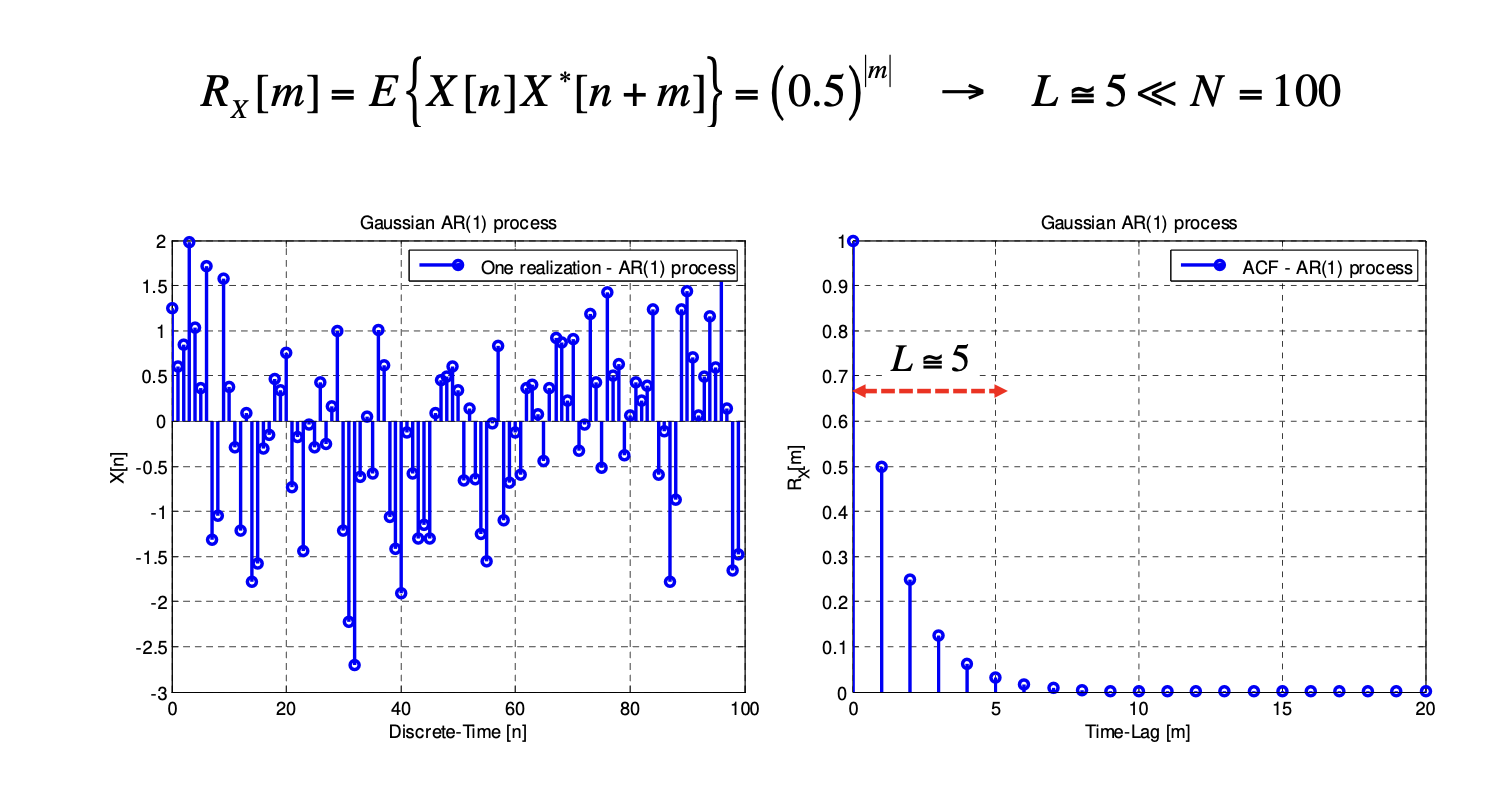
\includegraphics[width=1\linewidth]{Image/chap 1/7.Example.png}
\end{figure}
\subsubsection{IMPORTANT EXAMPLE}
\[
X(t)=A\cos(2\pi f_0t+\theta)+W(t),\hspace{0.25em}t\in[0,T),\hspace{0.5em}S_W(f)=\frac{N_0}{2}
\]
\noindent Where \(X(t)=s(t)+W(t)\) and the second one is an Additive white gaussian noise(AWGN)
\begin{itemize}
    \item A typical problem is to estimate the signal parameters (amplitude and phase) based on the observation of a noise corrupted version of the signal in the interval \([0,T)\).
    \item The signal frequency \(f_0\) may be a priori known or unknown. Let's assume first that it is a \underline{a-priori known}.
    \item After anti-aliasing filtering with bandwidith \(B=1/(2T_c)\) and ADC:
    \[
X[n] = A \cos \left( 2\pi F_0 n + \theta \right) + W[n], \quad n = 0, 1, \ldots, N-1
\]
\[
\text{where} \quad
F_0 \triangleq f_0 T_c \in (0, 1/2), \qquad
N = T/T_c = 2BT, \qquad
W[n] \in \mathcal{N}\left(0, \sigma_w^2 \right) \text{ IID}
\]
   \item The noise samples are independent and identically distributed.
   \item The discrete-time signal obtained by sampling can be expanded on the orthonormal basis functions as follows:
   \[
\begin{aligned}
X[n] &= A \cos \left( 2\pi F_0 n + \theta \right) + W[n] \\
     &= A \cos(\theta) \cos(2\pi F_0 n) - A \sin(\theta) \sin(2\pi F_0 n) + W[n] \\
     &= \sqrt{\frac{N}{2}} A \cos(\theta) \varphi_0[n]
        - \sqrt{\frac{N}{2}} A \sin(\theta) \varphi_1[n]
        + W[n]
\end{aligned}
\]
   \item Where:
   \[
\varphi_0[n] \triangleq \sqrt{\frac{2}{N}}\cos(2\pi F_0 n), \qquad
\varphi_1[n] \triangleq \sqrt{\frac{2}{N}}\sin(2\pi F_0 n), \qquad n=0,1,\ldots,N-1
\]

\[
(\varphi_i, \varphi_k) \triangleq \sum_{n=0}^{N-1} \varphi_i[n]\varphi_k^*[n] = \delta_{i,k} \quad \text{(Kronecker's delta)} \iff N \gg 1
\]

   \item In fact, if \(N\gg 1\):
   
   \[
(\varphi_0, \varphi_0) = \sum_{n=0}^{N-1} \sqrt{\frac{2}{N}}\cos(2\pi F_0 n) \sqrt{\frac{2}{N}}\cos(2\pi F_0 n)
= \frac{2}{N} \sum_{n=0}^{N-1} \cos^2(2\pi F_0 n)
\]
\[
= \frac{2}{N} \sum_{n=0}^{N-1} \left( \frac{1}{2} + \frac{1}{2}\cos(4\pi F_0 n) \right)
= 1 + \frac{1}{N} \sum_{n=0}^{N-1} \cos(4\pi F_0 n) \cong 1 \quad (\text{for } N \text{ very large})
\]
\[
(\varphi_1, \varphi_1) = \sum_{n=0}^{N-1} \sqrt{\frac{2}{N}}\sin(2\pi F_0 n) \sqrt{\frac{2}{N}}\sin(2\pi F_0 n)
= \frac{2}{N} \sum_{n=0}^{N-1} \sin^2(2\pi F_0 n)
\]
\[
= \frac{2}{N} \sum_{n=0}^{N-1} \left( \frac{1}{2} - \frac{1}{2}\cos(4\pi F_0 n) \right)
= 1 - \frac{1}{N} \sum_{n=0}^{N-1} \cos(4\pi F_0 n) \cong 1
\]
\[
(\varphi_0, \varphi_1) = \sum_{n=0}^{N-1} \sqrt{\frac{2}{N}}\cos(2\pi F_0 n) \sqrt{\frac{2}{N}}\sin(2\pi F_0 n)
= \frac{2}{N} \sum_{n=0}^{N-1} \frac{1}{2}\sin(4\pi F_0 n)
= \frac{1}{N} \sum_{n=0}^{N-1} \sin(4\pi F_0 n) \cong 0
\]
\item The other \(N-2\) orthonormal basis functions should be chosen to be unit-norm and orthogonal to the first two(we do not need to specify them).
\item The discrete-time signal can be expanded by using an orthonormal basis set and the coefficients of the expansion are derived as follows:
\[
    \alpha_k = \left( X[n], \varphi_k[n] \right ) = \sum_{n=0}^{N-1} X[n] \varphi_k^*[n] 
\]
\[ 
    \mathbf{a} = \begin{bmatrix} \alpha_0& \alpha_1 &\cdots & \alpha_{N-1}
\end{bmatrix}^T     
\]
\[
    \alpha_k = \left( X[n], \varphi_k[n] \right ) = \sum_{n=0}^{N-1} X[n] \varphi_k^*[n]
\]
\[
    = \sum_{n=0}^{N-1} \left( \sqrt{\frac{N}{2}} A \cos(\theta) \varphi_0[n] 
        - \sqrt{\frac{N}{2}} A \sin(\theta) \varphi_1[n]
        + W[n] \right) \varphi_k^*[n] \]
\[
    = \sqrt{\frac{N}{2}} A \cos(\theta) \sum_{n=0}^{N-1} \varphi_0[n] \varphi_k^*[n]
        - \sqrt{\frac{N}{2}} A \sin(\theta) \sum_{n=0}^{N-1} \varphi_1[n] \varphi_k^*[n]
        + \sum_{n=0}^{N-1} W[n] \varphi_k^*[n]
\]
\[
\alpha_k = \sqrt{\frac{N}{2}} A\cos(\theta)\delta_{0,k}
    - \sqrt{\frac{N}{2}} A\sin(\theta)\delta_{1,k}
    + W_k,\quad k = 0, 1, \cdots, N-1
\]
\item Where: \[W_k\triangleq(W[n],\varphi[n])=\sum_{n=0}^{N-1}W[n]\varphi_k^*[n]\]
Remeber that \(E\{W_k\}=0\).
\[
\mathbf{\alpha} = \mathbf{s} + \mathbf{w} =
\begin{bmatrix}
    \sqrt{\frac{N}{2}} A\cos(\theta) \\
    -\sqrt{\frac{N}{2}} A\sin(\theta) \\
    0 \\
    \vdots \\
    0
\end{bmatrix}
+
\begin{bmatrix}
    W_0 \\
    W_1 \\
    W_2 \\
    \vdots \\
    W_{N-1}
\end{bmatrix}
\]
\[
E\left\{ W_k W_i^* \right\} =
E\left\{ \sum_{n=0}^{N-1} W[n] \varphi_k^*[n] \sum_{l=0}^{N-1} W^*[l] \varphi_i[l] \right\}
\]
\[
= \sum_{n=0}^{N-1}\sum_{l=0}^{N-1} E\left\{ W[n] W^*[l] \right\} \varphi_i[l] \varphi_k^*[n]
\]
\[
= \sum_{n=0}^{N-1}\sum_{l=0}^{N-1} \sigma_w^2 \delta[n-l] \varphi_i[l] \varphi_k^*[n]
\]
\[
= \sigma_w^2 \sum_{n=0}^{N-1} \varphi_i[n] \varphi_k^*[n] = \sigma_w^2 \delta_{i,k}
\]
\[
\Rightarrow \quad W_k \in \mathcal{N}\left(0, \sigma_w^2 \right)\quad \text{IID}, \qquad \text{where}\quad \sigma_w^2 = \frac{N_0}{2 T_c} = 2B \frac{N_0}{2} = N_0 B
\]
\end{itemize}
\noindent Only the first two componenets bring information on the amplitude and phase of the useful signal. The other components are \textbf{irrelevant}, so we do not need to compute them:
\[
\alpha_0 = \left( X[n], \varphi_0[n] \right ) = \sqrt{\frac{2}{N}} \sum_{n=0}^{N-1} X[n] \cos(2\pi F_0 n)
\]
\[
\alpha_1 = \left( X[n], \varphi_1[n] \right ) = \sqrt{\frac{2}{N}} \sum_{n=0}^{N-1} X[n] \sin(2\pi F_0 n)
\]

\noindent This operation is equivalent to the extraction of the \textbf{In-phase(I)} and \textbf{Quadrature (Q) components}, typically called "\textbf{demodulation}", but in digital fashion, after the ADC.\\

\noindent Note tha the components of the transformed vector \(\alpha\) are uncorrelated:
\[
\mathbf{\alpha} =
\begin{bmatrix}
    \alpha_0 \\
    \alpha_1 \\
    \alpha_2 \\
    \vdots \\
    \alpha_{N-1}
\end{bmatrix}
=
\begin{bmatrix}
    \sqrt{\frac{N}{2}} A \cos(\theta) \\
    -\sqrt{\frac{N}{2}} A \sin(\theta) \\
    0 \\
    \vdots \\
    0
\end{bmatrix}
+
\begin{bmatrix}
    W_0 \\
    W_1 \\
    W_2 \\
    \vdots \\
    W_{N-1}
\end{bmatrix}
\quad \rightarrow \quad E\{\mathbf{\alpha}\} = E\{\mathbf{s} + \mathbf{W}\} = \mathbf{s}
\]

\[
\text{cov}(\alpha_k, \alpha_i) = E \left\{ (\alpha_k - s_k) (\alpha_i - s_i)^* \right\} = E \left\{ W_k W_i^* \right\} = \sigma_w^2 \delta_{i,k}
\]

\[
\Rightarrow \quad \text{cov}(\alpha_k, \alpha_i) = 0 \quad \text{for} \quad i \neq k
\]
The correlation matrix of vector \(\alpha\) is given by:
\[
\mathbf{R}_{\alpha} = E\{\mathbf{a} \mathbf{a}^H\} =
\begin{bmatrix}
    \sigma_0^2 & r_{01} & \cdots & 0 \\
    r_{10} & \sigma_1^2 & \cdots & 0 \\
    \vdots & \vdots & \ddots & \vdots \\
    0 & 0 & \cdots & \sigma_{N-1}^2
\end{bmatrix}
= \mathbf{C}_{\alpha} + \mathbf{n}_{\alpha} \mathbf{n}_{\alpha}^H = \sigma_w^2 \mathbf{I} + \mathbf{s} \mathbf{s}^H
\]

\[
r_{01} = r_{10} = E\left\{ \alpha_1 \alpha_0^* \right\} = E\left\{ \alpha_1 \right\} E\left\{ \alpha_0^* \right\} = s_1 s_0^* = -\frac{N A^2}{2}\cos(\theta)\sin(\theta) = -\frac{N A^2}{4}\sin(2\theta)
\]

\[
\sigma_i^2 = E\left\{|\alpha_i|^2\right\} = E\left\{ |s_i + W_i|^2 \right\} = |s_i|^2 + E\left\{ |W_i|^2 \right\} = |s_i|^2 + \sigma_w^2
\]

\[
\underbrace{\sigma_0^2 = \frac{N A^2}{2}\cos^2(\theta) + \sigma_w^2,\quad
\sigma_1^2 = \frac{N A^2}{2}\sin^2(\theta) + \sigma_w^2}_{\text{Pricipal components}},\quad
\sigma_i^2 = \sigma_w^2 \quad \text{per } 2 \leq i \leq N-1
\]
Block diagram where the \textbf{inner product(correlation)} is implemented digitally:
\begin{figure}[H]
    \centering
    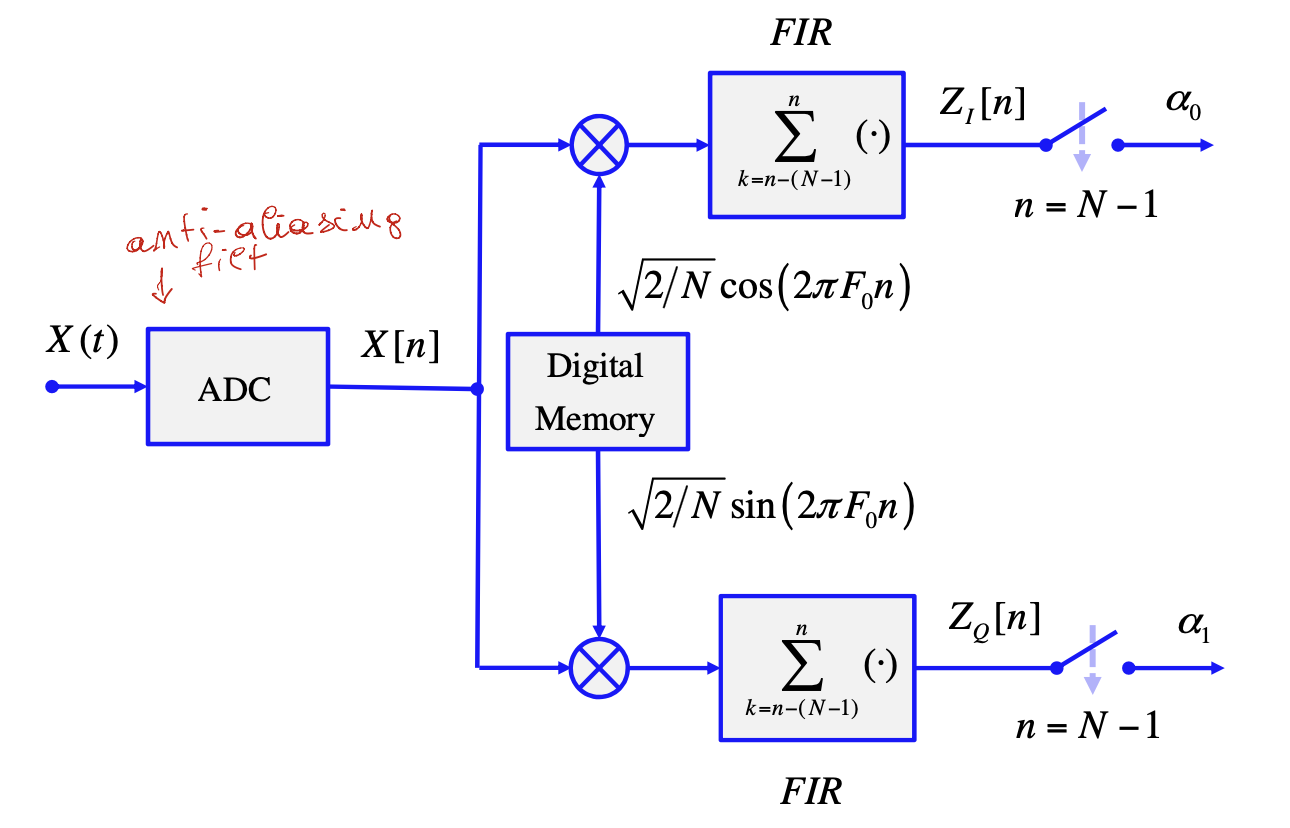
\includegraphics[width=0.75\linewidth]{Image/chap 1/8. Block_diag.png}
\end{figure}
Alternative approach: \textbf{correlator} structure that uses an analog \textbf{moving window integrator(MWI)}
\begin{figure}[H]
    \centering
    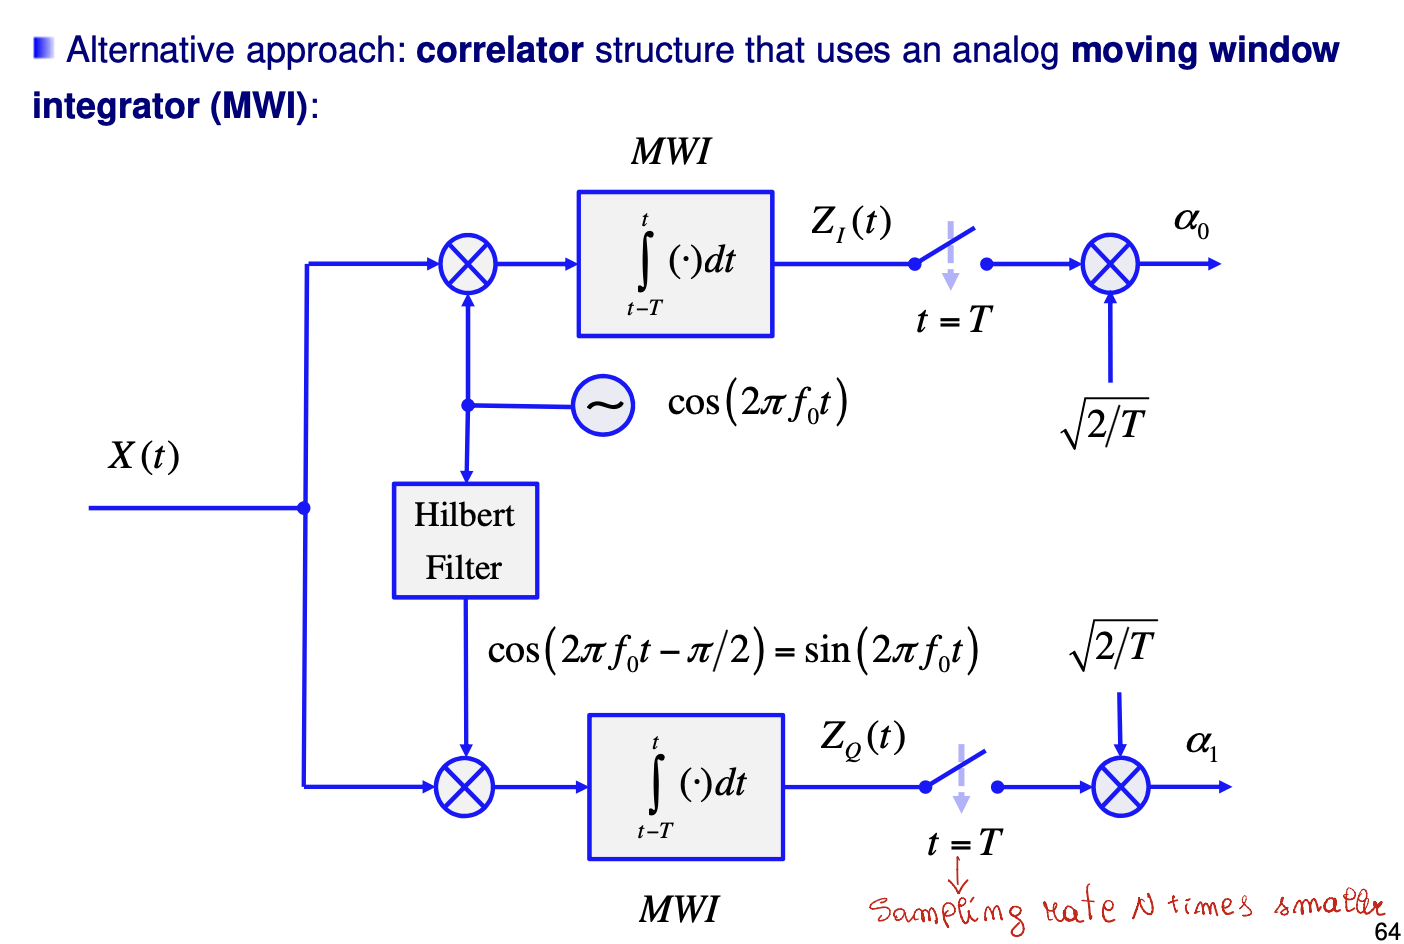
\includegraphics[width=0.75\linewidth]{Image/chap 1/9. Block_diag_MWI.png}
\end{figure}
\noindent \textbf{Typical approach}: first sample (ADC conversion) to get a discrete-time signal and then expand it by using the discrete-time orthonormal basis functions:
\[
\varphi_0[n] = \sqrt{\frac{2}{N}} \cos(2 \pi F_0 n), \qquad
\varphi_1[n] = \sqrt{\frac{2}{N}} \sin(2 \pi F_0 n), \qquad
n = 0, 1, \cdots, N-1
\]
Only the first two components of the new image vector are relevant, i.e they are the two \textbf{principal components}, so the 2D image vector is:
\[
\mathbf{a} \triangleq
\begin{bmatrix}
    \alpha_0 \\
    \alpha_1
\end{bmatrix}
=
\begin{bmatrix}
    \sqrt{\frac{N}{2}} A\cos(\theta) \\
    -\sqrt{\frac{N}{2}} A\sin(\theta)
\end{bmatrix}
+
\begin{bmatrix}
    W_0 \\
    W_1
\end{bmatrix}
= \mathbf{s} + \mathbf{W}
\]
\begin{itemize}
    \item The components \(\alpha_0\) and \(\alpha_1\) are typically called the \textbf{In-phase(I)} and \textbf{Quadrature (Q) components} with respect to the frequency \(f_0\).
    \item if \(N=2BT\gg 1\) the two approaches to extract the I \& Q components are equivalent from the point of view of \textbf{SNR}.
    \item The first approach is usually preferred because more efficient in terms of computational complexity (down-conversion to baseband, i.e extraction of the I \& Q components, is done digitally).
\end{itemize}
\noindent Let's compare the two SNR:
\begin{itemize}
    \item Image vector \textbf{X} \(SNR_{IN}\):
    \[
X[n] = \sqrt{\frac{N}{2}} A \cos(\theta) \varphi_0[n]
     - \sqrt{\frac{N}{2}} A \sin(\theta) \varphi_1[n]
     + W[n]; \qquad n = 0, 1, \cdots, N-1
\]

\[
\text{where} \quad W[n] \in \mathcal{N} \left(0, \sigma_w^2 \right)\quad \text{IID}, \qquad
\sigma_w^2 = N_0 B, \qquad N = \frac{T}{T_c} = 2BT
\]

\[
\mathbf{X} = \sqrt{\frac{N}{2}} A \cos(\theta) \varphi_0
           - \sqrt{\frac{N}{2}} A \sin(\theta) \varphi_1
           + \mathbf{W}_X
           \qquad \text{where} \qquad \mathbf{W}_X \triangleq [W[0]\; W[1]\; \cdots\; W[N-1]]^T
\]
\[
SNR_{IN} = \frac{E\left\{\|s_x\|_2^2\right\}}{E\left\{\|W_x\|_2^2\right\}}
= \frac{ \|s_x\|_2^2 }{ E\left\{ \sum_{n=0}^{N-1} W^2[n] \right\} }
= \frac{ \left\| \sqrt{\frac{N}{2}} A\cos(\theta) \varphi_0 - \sqrt{\frac{N}{2}} A\sin(\theta) \varphi_1 \right\|_2^2 }
         { \sum_{n=0}^{N-1} E\left\{ W^2[n] \right\} }
\]
\[
= \frac{
  \frac{N A^2}{2} \cos^2(\theta) \|\varphi_0\|_2^2
+ \frac{N A^2}{2} \sin^2(\theta) \|\varphi_1\|_2^2
- 2\cdot \frac{N A^2}{2} \cos(\theta)\sin(\theta) (\varphi_0,\varphi_1)
}{
  N \sigma_w^2
}
\]
\[
= \frac{
  \frac{N A^2}{2} \cos^2(\theta) + \frac{N A^2}{2} \sin^2(\theta)
}{
  N \sigma_w^2
}
= \frac{A^2}{2 \sigma_w^2}
\]
\item SNR for the transformed image vector \(\alpha\) \(SNR_{OUT}\)
\[
\mathbf{a} =
\begin{bmatrix}
    \alpha_0 \\
    \alpha_1
\end{bmatrix}
=
\begin{bmatrix}
    \sqrt{\frac{N}{2}} A \cos(\theta) \\
    -\sqrt{\frac{N}{2}} A \sin(\theta)
\end{bmatrix}
+
\begin{bmatrix}
    W_0 \\
    W_1
\end{bmatrix}
= \mathbf{s} + \mathbf{W}, \quad
\text{where} \quad W_k \in \mathcal{N}(0,\sigma_w^2),\quad \text{IID}
\]

\[
SNR_{OUT} = \frac{E\left\{ \|\mathbf{s}\|_2^2 \right\}}{E\left\{ \|\mathbf{W}\|_2^2 \right\}}
= \frac{ s_0^2 + s_1^2 }{ E\left\{ W_0^2 + W_1^2 \right\} }
= \frac{A^2 N / 2}{2\sigma_w^2}
= \frac{A^2 N / 2}{2 \cdot N_0 B}
= \frac{A^2 T}{2 N_0}
= \frac{E_s}{N_0}
\]
\item The \textbf{Processing gain(PG)} is the gain in SNR that we achieve thanks to the linear transformation:
\[
PG=\frac{SNR_{OUT}}{SNR_{IN}}=\frac{A^2N/2}{2\sigma^2_W}\Big{/}\frac{A^2}{2\sigma_W^2}=\frac{N}{2}
\]
\newpage
\item Calculations of the two principal components is equivalent to calculating the \textbf{DTFT} of the observed signal \(X[n]\) at the digital frequency \(F_0\), which is the most powerful frequency component present in the \textit{Sol} \(s[n]\) observed in \([0,T)\):
\[
\alpha_0 = \sqrt{\frac{2}{N}} \sum_{n=0}^{N-1} X[n] \cos(2\pi F_0 n)
= \sqrt{\frac{2}{N}}\, \Re \left\{ \sum_{n=0}^{N-1} X[n] e^{-j 2\pi F_0 n} \right\}
= \sqrt{\frac{2}{N}}\, \Re \left\{ DTFT\left( \mathbf{X} \right) \Big|_{F=F_0} \right\}
\]
\[
\alpha_1 = \sqrt{\frac{2}{N}} \sum_{n=0}^{N-1} X[n] \sin(2\pi F_0 n)
= -\sqrt{\frac{2}{N}}\, \Im \left\{ \sum_{n=0}^{N-1} X[n] e^{-j 2\pi F_0 n} \right\}
= -\sqrt{\frac{2}{N}}\, \Im \left\{ DTFT\left( \mathbf{X} \right) \Big|_{F=F_0} \right\}
\]
\end{itemize}
\[
X[n] = s[n] + W[n] = A \cos(2\pi F_0 n + \theta) + W[n], \qquad n = 0, 1, \cdots, N-1
\]

\[
S\left(e^{j 2\pi F}\right) = DTFT\{ s[n] \} = \sum_{n=0}^{N-1} s[n] e^{-j 2\pi F n}
\]

\[
PSD_S\left(e^{j 2\pi F}\right) = \lim_{N \to \infty} \frac{1}{N} \left| S\left(e^{j 2\pi F}\right) \right|^2
\]
\[
SNR(F)=\frac{PSD_S(e^{j2\pi F})}{PSD_W(e^{j2\pi F})} \qquad F_0=arg\max\{SNR(F)\}
\]\begin{figure}[H]
    \centering
    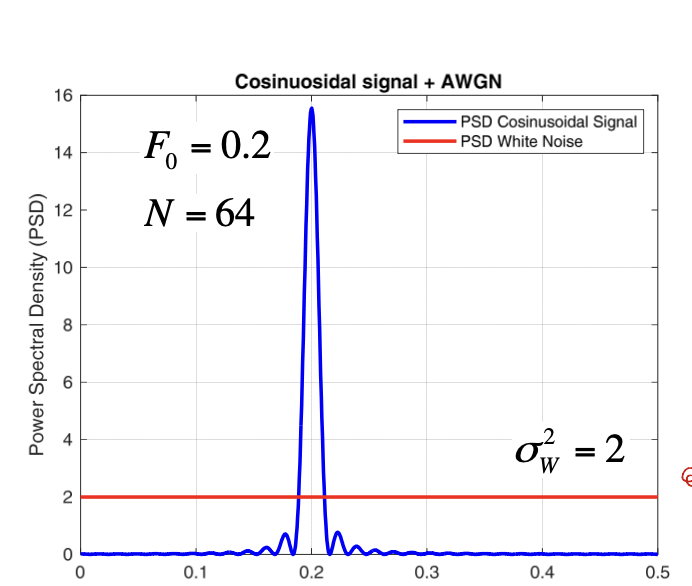
\includegraphics[width=0.5\linewidth]{Image/chap 1/10. PSD.png}

    \label{fig:placeholder}
\end{figure}
\[
\alpha_0 = \sqrt{\frac{2}{N}}\, \Re\left\{ DTFT\left(\mathbf{X}\right)\Big|_{F=F_0}\right\}
\qquad
\alpha_1 = -\sqrt{\frac{2}{N}}\, \Im\left\{ DTFT\left(\mathbf{X}\right)\Big|_{F=F_0}\right\}
\]
\begin{itemize}
    \item The values of the DTFT at frequencies different from \(F_0\) are not relevant, i.e. they do not bring additional useful information about the amplitude and phase of the signal of interest \(s[n]\).
    \item The two principal components \(\alpha_0\) and \(\alpha_1\) contains all the relevant information about the amplitude \(A\) and the phase \(\theta\) can be estimated from \(\alpha_0\) and \(\alpha_1\).
    \item This is possible if we know a \textit{a priori} the signal frequency \(F_0\)(remember that \underline{the basis functions should }\\
    \underline{be deterministic perfectly known}).
    \item If the signal frequency \(F_0\) is unknown:\\
    We use the FFT to calculate the DTFT of the \(N-\)dimensional vector \(\textbf{X}\) at all the discrete frequencies \(F_k=k/N\) (or \(F_k=k/N_{zp}\) if we use zero-padding) and then we select the two principal components, i.e. the real and imaginary parts of the FFT at the frequency for which the \(|FFT|^2\) assumes the greates values.
\end{itemize}

\clearpage